\documentclass{article}

% Language setting
% Replace `english' with e.g. `spanish' to change the document language
\usepackage[english]{babel}

% Set page size and margins
% Replace `a4paper' with `letterpaper' for USA and Americas standard size
\usepackage[a4paper,top=2cm,bottom=2cm,left=3cm,right=3cm,marginparwidth=1.75cm]{geometry}

% Useful packages
\usepackage{amsmath}
\usepackage{graphicx}
\usepackage[colorlinks=true, allcolors=blue]{hyperref}
\usepackage{makecell}

\title{% 
    \textbf{Master Thesis Research Proposal}\\
    \vfill
    \textbf{Your Title Goes Here}
    }
\author{Your Full Name}

\begin{document}
\maketitle

{\centering
    Supervisor: [Your Supervisor(s) name]\\
    \vfill
    Tallinn University / Cyprus University of Technology\\
    \href{mailto: youremail@idmaster.eu}{youremail@idmaster.eu}\\ %Change both email fields!
    }

\begin{abstract}
Your abstract goes here. One paragraph that summarizes the content of your proposal. Begin with one or two sentences of your research problem. Then present your motivation and your insight about how to address it. Then present your research goal and methods and your expected outcomes.
\vfill
\textbf{Keywords:} 4-5 Keywords, separated by commas.
\end{abstract}


\section{Introduction}
A small introduction presenting the main idea, rationale, and background of the proposal. It serves to introduce the topic, scope and research perspective to the reader and sets up the expectations for the following sections. It is recommended that the basic assertions are supported by references.

This template is prepared in Overleaf. To view tutorials, user guides, and further documentation, please visit our \href{https://www.overleaf.com/learn}{help library}, or head to our plans page to \href{https://www.overleaf.com/user/subscription/plans}{choose your plan}. Or just write me at \href{mailto: dirabien@tlu.ee}{dirabien@tlu.ee} or Mustafa at \href{mailto: rajaz@tlu.ee}{rajaz@tlu.ee}.

\section{Problem Statement}
States the research problem, gives evidence that it is in fact a research problem.
Discusses the current state of the art in the research field. This includes a critical summary and discussion of previous attempts to solve the research problem by other researchers and gives appropriate citations to that work.
Mentions the contribution of the current proposal to this problem.

\subsection{Research Motivation and Purpose}

Explain simply and clearly what's your motivation to address this problem and what is the purpose of your research. Why is this important?

\subsection{How to create Sections and Subsections}

Simply use the section and subsection commands, as in this example document! With Overleaf, all the formatting and numbering is handled automatically according to the template you've chosen. If you're using Rich Text mode, you can also create new section and subsections via the buttons in the editor toolbar.

\section{Literature Review}
A summary of the literature review you conducted. It introduces the related work and conceptual framework that supports the proposed research problem.
It should give a solid summary of the state-of-the-art on the topic and identify the relevant gap or need that the proposal aims to address.
While it doesn’t need to be systematic, it should be deep and show that the author has a deep understanding of the main ideas and problems on the topic. It should not be a simple list of references and highlights but an intellectual engagement with the materials showing the author’s take on the literature.

\subsection{How to add Citations and a References List}

You can simply upload a \verb|.bib| file containing your BibTeX entries, created with a tool such as Zotero, Mendeley, Paperpile orJabRef. You can then cite entries from it, like this: \cite{viNotJustSeeing2017}. Just remember to specify a bibliography style, as well as the filename of the \verb|.bib|. You can find a \href{https://www.overleaf.com/help/97-how-to-include-a-bibliography-using-bibtex}{video tutorial here} to learn more about BibTeX.

Just to have one, we can add a couple more of citations, like \cite{lempinenConstructingDesignFramework2012}, \cite{menichinelliResearchDesignFramework2019} and \cite{andersonFrameworkDevelopingAlternative2021}. Here is one of the biggest advantages of \LaTeX: \hspace{1pt} It allows us to add our references and forget about doing the Reference list manually and mess with the formats. We can even easily change the bibliographic format we use! In my case, since I am very prone to forget things, this is a kill feature.

\section{Research Goal and Research Questions}
States the goal / objective / purpose of the research that is derived from the problem statement
Lists concrete, specific questions stated in operational terms that can be answered with the research

\subsection{Research Questions}
Here you present your Research Questions
\begin{enumerate}
    \item \textit{ What is your Research Question?}
    \item \textit{Do you have more than One?}
\end{enumerate}

\subsection{How to add Lists}

You can make lists with automatic numbering \dots
\begin{enumerate}
\item Like this,
\item and like this.
\end{enumerate}
\dots or bullet points \dots
\begin{itemize}
\item Like this,
\item and like this.
\end{itemize}

\section{Conceptual or Theoretical Framework (if needed) and Methodology}
If you are working with some specific Framework, you introduce the framework, the rationale for selecting it for this proposal and how you plan to engage with it for your research.
You present the general Research Methodology (e.g. Design Research, Experimental Research, Qualitative, Quantitative, Mixed Methods, Constructivism, Etc …) that you plan to use, and how it relates to the methods that you are selecting to answer your Research Question(s)
Describes the Sample, the Methods, the Materials and Procedures used and the implementation. If you have more than one Research Question it is a good practice to create a table or section where you explain which method(s) are being used for answering which Research Questions.
Remember that you have Methods for Data Collection and Methods for Data Analysis. You should explain not only how you are going to collect the data but also how you plan to analyze it.

\subsection{How to add Tables}

Use the table and tabular environments for basic tables --- see Table~\ref{tab:research design}, for example. For more information, please see this help article on \href{https://www.overleaf.com/learn/latex/tables}{tables}. 

Tables in \LaTeX \hspace{1pt} are not so straightforward as in other places. If you prefer, you can prepare them in other sources and paste them as figures, although that would limit our ability to select text in them. But if you are ready for a challenge, just jump in!

In the Source View you can find the code for our Table 1. The first row of data will always be the Header and the rest will be the content. You have to manually manage the length of the cells, since \LaTeX \hspace{1pt} won't do it on its own (it had to have one little thing). 

To manage it so, we are using an extra package called makecell that allows us to use some extra formatting options. The two new commands we use are \verb+\thead{}+ for the headers and \verb+\makecell()+ for the cells. This allows us add breaks to the cells without messing our table. 

Finally, one last note to understand, the command \verb+\begin{tabular}{c|c}+ begins with just one vertical line | and two c's. This letter refers to the alignment, l for left and r right. The | is to indicate where you want a vertical line. You can add as many rows as you want by adding vertical lines and l,c or r to the the keys after the tabular command.

Yes, it is a bit convoluted but the ONE thing it does amazing, is that it numbers correctly all your tables and references automatically. Making adding and editing very easy and reducing the risk of silly errors. So it is worth a try. Again, if you have any doubts you can ask us.

\begin{table}[htb] %NB: The [htb] argument is what makes the table appear after the text talking about the table. If we don't use it, the table can appear before if this is the most suitable position for it. 
\centering
\begin{tabular}{|c|c|c|c|c|c|}
\hline %This adds an horizontal line to the top of the table.
\thead{\textbf{Phase}} & \thead{\textbf{Study}} & \thead{\textbf{Objectives}} 
& \thead{\textbf{Data Collection}\\\textbf{Methods}} 
& \thead{\textbf{Data Analysis}\\ \textbf{Methods}} 
& \thead{\textbf{Expected} \\\textbf{Outcome}} \\ \hline %The \\ is the linebreak 

I & \makecell{Conceptual \\ Wizard of Oz} & \makecell{Validating \\initial \\ concept}
& \makecell{Unstructured\\Interviews} & \makecell{Qualitative \\Content \\ Analysis} 
& \makecell{Design Artifact\\ Guidelines} \\\hline 

II & \makecell{Low-Fi Prototype \\ Case Study} & \makecell{Addressing\\RQ1}
& \makecell{Semi-structured\\Interviews} & \makecell{Qualitative \\Content \\ Analysis} 
& \makecell{Initial \\ Understanding\\ of RQ1} \\\hline 

III & \makecell{Hi-Fi Prototype \\ Case Study} & \makecell{Addressing\\RQ1}
& \makecell{Semi-structured\\Interviews} & \makecell{Qualitative \\Content \\ Analysis} 
& \makecell{In-Depth \\ Understanding\\ of RQ1} \\\hline 

III & \makecell{2nd Iteration \\ Hi-Fi Prototype \\ Case Study} & \makecell{Addressing\\RQ1}
& \makecell{Semi-structured\\Interviews} & \makecell{Qualitative \\Content \\ Analysis} 
& \makecell{In-Depth \\ Understanding\\ of RQ1} \\\hline 

\end{tabular}
\caption{\label{tab:research design}Example of a Table with and Example of a Research Design.}
\end{table}

% if you must use one, here is the command to "encourage" the system to use one. It will still not use it if it is not a good idea.

%\pagebreak 

\section{Research Plan}
Mentions the time plan, resources needed and constraints that the research faces and possibilities to overcome them.
It is strongly recommended to add a Gantt chart illustrating the schedule of the plan.


\subsection{How to include Figures}

First you have to upload the image file from your computer using the upload link in the file-tree menu. Then use the includegraphics command to include it in your document. Use the figure environment and the caption command to add a number and a caption to your figure. See the code for Figure \ref{fig:research plan} in this section for an example.

Note that your figure will automatically be placed in the most appropriate place for it, given the surrounding text and taking into account other figures or tables that may be close by. You can find out more about adding images to your documents in this help article on \href{https://www.overleaf.com/learn/how-to/Including_images_on_Overleaf}{including images on Overleaf}.

\begin{figure}[htb]
\centering
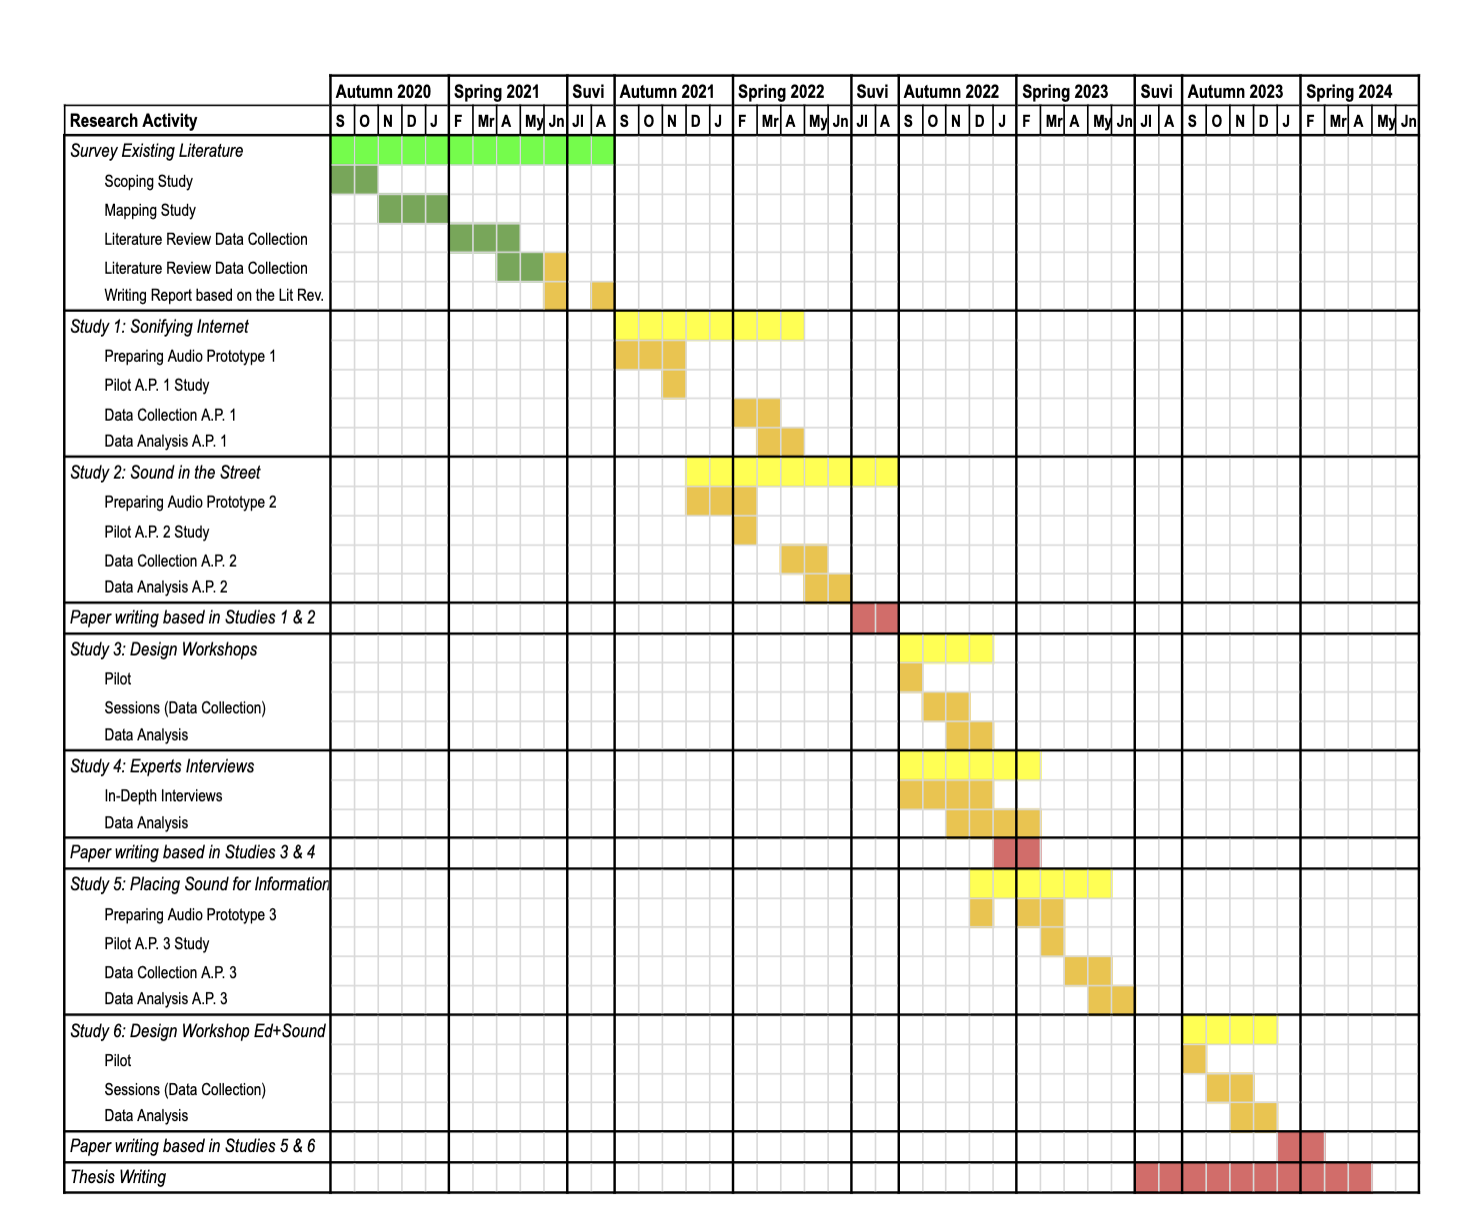
\includegraphics[width=0.3\textwidth]{Gantt Chart.png}
\caption{\label{fig:research plan}A very optimistic Research Plan}
\end{figure}

\section{Expected Outcomes}
Presents the expected outcomes from the work. It has to be aligned with the previous sections and Proposal Goals

\section{Conclusions}
A brief closing statement rounding up the proposal.

\subsection{How to add Comments and Track Changes}

Comments can be added to your project by highlighting some text and clicking ``Add comment'' in the top right of the editor pane. To view existing comments, click on the Review menu in the toolbar above. To reply to a comment, click on the Reply button in the lower right corner of the comment. You can close the Review pane by clicking its name on the toolbar when you're done reviewing for the time being.

Track changes are available on all our \href{https://www.overleaf.com/user/subscription/plans}{premium plans}, and can be toggled on or off using the option at the top of the Review pane. Track changes allow you to keep track of every change made to the document, along with the person making the change. 

\bibliographystyle{acm}
\bibliography{sample}

\end{document}